\documentclass[english,floatsintext,man]{apa6}

\usepackage{amssymb,amsmath}
\usepackage{ifxetex,ifluatex}
\usepackage{fixltx2e} % provides \textsubscript
\ifnum 0\ifxetex 1\fi\ifluatex 1\fi=0 % if pdftex
  \usepackage[T1]{fontenc}
  \usepackage[utf8]{inputenc}
\else % if luatex or xelatex
  \ifxetex
    \usepackage{mathspec}
    \usepackage{xltxtra,xunicode}
  \else
    \usepackage{fontspec}
  \fi
  \defaultfontfeatures{Mapping=tex-text,Scale=MatchLowercase}
  \newcommand{\euro}{€}
\fi
% use upquote if available, for straight quotes in verbatim environments
\IfFileExists{upquote.sty}{\usepackage{upquote}}{}
% use microtype if available
\IfFileExists{microtype.sty}{\usepackage{microtype}}{}

% Table formatting
\usepackage{longtable, booktabs}
\usepackage{lscape}
% \usepackage[counterclockwise]{rotating}   % Landscape page setup for large tables
\usepackage{multirow}		% Table styling
\usepackage{tabularx}		% Control Column width
\usepackage[flushleft]{threeparttable}	% Allows for three part tables with a specified notes section
\usepackage{threeparttablex}            % Lets threeparttable work with longtable

% Create new environments so endfloat can handle them
% \newenvironment{ltable}
%   {\begin{landscape}\begin{center}\begin{threeparttable}}
%   {\end{threeparttable}\end{center}\end{landscape}}

\newenvironment{lltable}
  {\begin{landscape}\begin{center}\begin{ThreePartTable}}
  {\end{ThreePartTable}\end{center}\end{landscape}}




% The following enables adjusting longtable caption width to table width
% Solution found at http://golatex.de/longtable-mit-caption-so-breit-wie-die-tabelle-t15767.html
\makeatletter
\newcommand\LastLTentrywidth{1em}
\newlength\longtablewidth
\setlength{\longtablewidth}{1in}
\newcommand\getlongtablewidth{%
 \begingroup
  \ifcsname LT@\roman{LT@tables}\endcsname
  \global\longtablewidth=0pt
  \renewcommand\LT@entry[2]{\global\advance\longtablewidth by ##2\relax\gdef\LastLTentrywidth{##2}}%
  \@nameuse{LT@\roman{LT@tables}}%
  \fi
\endgroup}


  \usepackage{graphicx}
  \makeatletter
  \def\maxwidth{\ifdim\Gin@nat@width>\linewidth\linewidth\else\Gin@nat@width\fi}
  \def\maxheight{\ifdim\Gin@nat@height>\textheight\textheight\else\Gin@nat@height\fi}
  \makeatother
  % Scale images if necessary, so that they will not overflow the page
  % margins by default, and it is still possible to overwrite the defaults
  % using explicit options in \includegraphics[width, height, ...]{}
  \setkeys{Gin}{width=\maxwidth,height=\maxheight,keepaspectratio}
\ifxetex
  \usepackage[setpagesize=false, % page size defined by xetex
              unicode=false, % unicode breaks when used with xetex
              xetex]{hyperref}
\else
  \usepackage[unicode=true]{hyperref}
\fi
\hypersetup{breaklinks=true,
            pdfauthor={},
            pdftitle={Race-based disparities in allocation of academic disciplinary actions are associated with county-level rates of bias},
            colorlinks=true,
            citecolor=blue,
            urlcolor=blue,
            linkcolor=black,
            pdfborder={0 0 0}}
\urlstyle{same}  % don't use monospace font for urls

\setlength{\parindent}{0pt}
%\setlength{\parskip}{0pt plus 0pt minus 0pt}

\setlength{\emergencystretch}{3em}  % prevent overfull lines

\ifxetex
  \usepackage{polyglossia}
  \setmainlanguage{}
\else
  \usepackage[english]{babel}
\fi

% Manuscript styling
\captionsetup{font=singlespacing,justification=justified}
\usepackage{csquotes}
\usepackage{upgreek}

 % Line numbering
  \usepackage{lineno}
  \linenumbers


\usepackage{tikz} % Variable definition to generate author note

% fix for \tightlist problem in pandoc 1.14
\providecommand{\tightlist}{%
  \setlength{\itemsep}{0pt}\setlength{\parskip}{0pt}}

% Essential manuscript parts
  \title{Race-based disparities in allocation of academic disciplinary actions
are associated with county-level rates of bias}

  \shorttitle{Discipline Disparities}


  \author{Travis Riddle\textsuperscript{1}~\& Stacey Sinclair\textsuperscript{1}}

  \def\affdep{{"", ""}}%
  \def\affcity{{"", ""}}%

  \affiliation{
    \vspace{0.5cm}
          \textsuperscript{1} Princeton University  }

  \authornote{
    \newcounter{author}
    Enter author note here.

                      Correspondence concerning this article should be addressed to Travis Riddle. E-mail: \href{mailto:triddle@princeton.edu}{\nolinkurl{triddle@princeton.edu}}
                          }


  \abstract{Enter abstract here.}
  \keywords{keywords \\

    \indent Word count: X
  }





\usepackage{amsthm}
\newtheorem{theorem}{Theorem}
\newtheorem{lemma}{Lemma}
\theoremstyle{definition}
\newtheorem{definition}{Definition}
\newtheorem{corollary}{Corollary}
\newtheorem{proposition}{Proposition}
\theoremstyle{definition}
\newtheorem{example}{Example}
\theoremstyle{remark}
\newtheorem*{remark}{Remark}
\begin{document}

\maketitle

\setcounter{secnumdepth}{0}



\section{Introduction}\label{introduction}

In comparison to White Americans, African Americans exhibit poorer
educational outcomes across a range of metrics. One outcome of
particular concern is the gap in disciplinary actions (Kinsler, 2011;
Okonofua, Walton, \& Eberhardt, 2016). Research using administrative
datasets and longitudinal samples clearly show that African American
students are far more likely to be suspended or expelled (Aud,
KewalRamani, \& Frohlich, 2011; Yeager, Purdie-Vaughns, Hooper, \&
Cohen, 2017), and conditional on an office referral, are more likely to
receive stiffer punishments (J. F. Gregory, 1995). Concerns about these
disparities are exacerbated by their associations with long-term life
outcomes, including prospects for employment (Pager, Western, \& Sugie,
2009), mental and physical health (Pascoe \& Smart Richman, 2009), and
involvement in the criminal justice system (Hirschfield, 2009). In this
paper, we aim to establish that these disciplinary gaps are related to
environmental levels of bias in predictable ways.

It is perhaps not surprising that levels of bias would be associated
with racial disciplinary gaps. This straightforward statement, however,
is contextualized in a number of ways. First, the operationalization of
bias should play a role in the association. As we describe below, levels
of implicit and explicit biases should be differentially associated with
disciplinary actions. This differential association should be
determined, in part, by the type of disciplinary action under
examination. For a given student committing a specific offense, the
educational institution may opt for one of several disciplinary actions.
These actions vary in severity, institutional costs, and the degree of
formal administrative involvement.

To illustrate this problem in the context of previous research, we now
describe research on the associations between implicit bias and explicit
bias and decision making. This sets the stage for understanding what
types of decisions administrators and educators make when electing a
specific disciplinary action. We then describe the types of disciplinary
actions that are taken and the characteristics of these actions in terms
of severity, institutional costs, and formal administrative involvement.
Finally, in crossing this information, we concretely specify the set of
associations expected when examining bias and disciplinary actions in
American schools.

\subsection{Bias and decision-making}\label{bias-and-decision-making}

Previous research on biased attitudes and behavior has shown that
although implicit and explicit attitudes are typically correlated
(Hofmann, Gawronski, Gschwendner, Le, \& Schmitt, 2005; McConnell \&
Leibold, 2001), they tend to behaviorally manifest slightly differently.
As a default, a naiive expectation is that explicit attitudes should
guide behavior, since if people tell us they like something, we should
expect that to generally correspond to their behavior. However, under
some circumstances, implicit biases are more strongly associated with
behavioral outcomes. B. A. Nosek, Hawkins, and Frazier (2011) suggest
that, in comparison to explicit attitudes, implicit attitudes are more
strongly associated with behavior when the individual lacks motivated to
explicitly respond differently than their implicit attitude would
suggest, when they do not have the opportunity or ability to modify
their initial response inclination, or when they do not have awareness
of the implicit response, the behavior, or the link between them. In
contrast, the more motivated, more able, or more aware the person is
over their behavioral response, the more explicit biases should play a
role. One key situational factor that determines the response is
situational uncertainty. In uncertain situations, the respondent is not
likely to have strong motivations to change their initial response,
otherwise the situation would not be uncertain. Research supports this
idea, as when the situation is characterized by greater uncertainty,
implicit biases are known to be stronger determinants of behavior
(Friese, Hofmann, \& Schmitt, 2009; Galdi, Arcuri, \& Gawronski, 2008;
Gawronski, Geschke, \& Banse, 2003). In short, when taking (or not
taking) an action can be attributed to multiple reasons due to
situational ambiguity, then implicit biases should result in higher
rates of discriminatory behavior.

Accordingly, this research suggests that disciplinary actions that are
implemented quickly, have relatively little administrative oversight,
and require little in the way of insitutional resources should be
characterized by strong associations with implicit bias. On the other
hand, any disciplinary action that requires higher levels of oversight,
resources, or lengthy time investments to complete should be more
strongly associated with explicit bias.

\subsection{Types of disciplinary
actions}\label{types-of-disciplinary-actions}

We report here on five different types of disciplinary actions:
in-school suspensions, out-of-school suspensions, law enforcement
referrals, school-related arrests, and expulsions. As described above,
these actions vary in severity, required resources, and administrative
oversight.

The most extreme outcome, expulsion, is defined as when a student is
prohibited from ever returning to the educational institution. The
institution may or may not set up alternative educational services for
the student. Because of the the severe nature of this punishment, it
also requires considerable administrative oversight, and is often
conferred for behaviors that are relatively unambiguous (e.g.~bringing a
gun to school). We believe similar cases can be made for law enforcement
referrals and school-related arrests insofar as these actions tend to be
more severe, and require resources, or occasionally the involvement of
outside agencies.

Somewhat less severe than expulsions, but one of the most frequently
utilized disciplinary actions, out-of-school suspensions occupy
something of a middle ground. There is a substantial body of research
documenting the negative associations between this particular
disciplinary action and life outcome (Cuellar \& Markowitz, 2015;
Matjasko, 2011), as well as their disproportionate use on stigmatized
students (Haight, Gibson, Kayama, Marshall, \& Wilson, 2014; Kinsler,
2011). Out-of-school suspensions are administered for a wide range of
behaviors. Some of these behaviors are apt to be determined with a fair
degree of subjectivity (e.g.~defiance) (A. Gregory \& Weinstein, 2008),
while others may be more unambiguous (e.g.~fighting, drug use). In
comparison to expulsions and arrests, this type of action demands less
administrative oversight.

In-school suspensions, wherein the student is removed from the classroom
but remains under the direct supervision of school personnel, are also
administered for a wide range of behaviors. However, in-school
suspensions have been highlighted as a promising alternative to more
exclusionary types of disciplinary actions (e.g.~out-of-school
suspensions, expulsions) partly because students remain under the
supervision of school personnel, which keeps them in a structured,
educational setting (Anyon et al., 2014). Like out-of-school
suspensions, this type of action requires relatively little
administrative oversight. But unlike out-of-school suspension, removing
a student from a classroom to a \emph{different} educational setting
requires additional space and personnel, and so this represents an
inherent investment in the student.

\subsection{Concrete predictions of
association}\label{concrete-predictions-of-association}

Given these disciplinary outcomes and what is known about implicit and
explicit attitudes, what should we expect in examining associations
between them? First, it's clear that we should expect African American
students to receive higher levels of disciplinary actions. Second, we
should expect the disparity in disciplinary actions to generally be
positively associated with explicit bias. Finally, we should expect
implicit bias to only show associations in instances where there is
little administrative overhead, and where the behaviors to-be-punished
are often ambiguous. By this logic, out-of-school suspensions are the
only metric that meet these criteria.

\subsection{The present study}\label{the-present-study}

The present study uses a national dataset of disciplinary outcomes to
evaluate the degree to which implicit and explicit bias are associated
with each of these outcomes. After an initial, registered analytic
approach, we subsequently made several adjustments to strengthen our
analyses and streamlined them with respect to previous research. In
general, the data support the conclusion that implicit biases are
specifically associated with out-of-school suspensions, while explicit
biases tend to be associated with disciplinary actions of all types.

\section{Methods}\label{methods}

\subsection{Data Sources}\label{data-sources}

\subsubsection{Disciplinary actions}\label{disciplinary-actions}

To assess rates of disciplinary action, we used data from the Civil
Rights Data Collection (CRDC) conducted by the US Department of
Education. The dataset we used comes from the 2013-2014 academic year
and has data on \enquote{all public local and educational agencies and
schools, including long-term secure juvenile justice facilities, charter
schools, alternative schools, and schools serving students with
disabilities.} In total, the CRDC data represents 95507 institutions
enrolling approximately 50 million students, of which approximately 25
million are white and 7.8 million are Black\footnote{We note that there
  are a number of differences between the analyses we registered and
  those presented in the main text. Our general conclusions are largely
  the same for both sets of analyses. We opted to report the modified
  analyses for reasons of clarity and to remain congruent with previous
  research on the same topics. The registered analyses can be found, in
  full, in the appendix.}. Previous work using these data have
identified a number of districts whose data are in error, and have
excluded juvenile justice facilities, as these institutions constitute
dramatically different educational environments, where the meaning of
disciplinary actions may be quite different (Losen et al., 2015). After
these exclusions are applied, the final sample used for modeling
consists of 90002 institutions, enrolling 32 million black or white
students, of which 24.70 million are white and 7.30 million are black.
From these data, we focus on the number of students by race (black and
white) who received one of several types of disciplinary action. We
report here rates of out-of-school suspension, in-school suspension,
school-related arrests, law enforcement referrals, and total number of
expulsions of any type.

\subsubsection{Racial Bias}\label{racial-bias}

We used measurements of implicit and explicit bias available from data
collected through Project Implicit (Xu, Nosek, \& Greenwald, 2014). For
a full description of the implicit and explicit bias measures available
in these data, refer to Xu et al. (2014) and Leitner, Hehman, Ayduk, and
Mendoza-Denton (2016). We note only that we used the IAT D-score as a
measure of implicit bias, and the difference between reported warmth
towards whites and warmth towards black (both measured from 0=very cold,
10=very warm) as a measure of explicit bias. Additionally, we used only
respondents who had geographic information that would allow us to place
them in a United States county, identified as White, and visited the
site before 2015. This consisted of approximately 1.1 million total
respondents from 3091 counties.

\subsubsection{Covariates}\label{covariates}

Each county-level variable used as a covariates in the final model and
the corresponding state-level variable used as a predictor in the
post-stratification scheme were taken from the from the same source.
Population size and proportions, socioeconomic indicators, and mobility
were all taken from the American Community Survey (ACS) 5-year estimates
for the time period ending in 2014. Urban-rural indicators were taken
from the 2010 US Census, and crime rates were taken from the FBI Uniform
Crime Reporting program, as made available through the National Archive
of Criminal Justice Data for each year from 2010-2014. Each of these
variables is described below.

\paragraph{Population size and
proportions}\label{population-size-and-proportions}

We obtained the total population, the proportion of the population that
is white, the proportion of the population that is black, and the ratio
of black-to-white people in the population from ACS table B02001.

\paragraph{Socioeconomic indicators}\label{socioeconomic-indicators}

We obtained estimates for the percentage of population with a Bachelor's
degree or higher, the percentage of the population aged 16 or over in
the labor force that is unemployed, the median household income, and the
percentage of families and people whose income in the last year was
below the poverty line from the ACS table DP03.

\paragraph{Urban-rural indicator}\label{urban-rural-indicator}

We obtained estimates of housing density per square mile of land area
from Census table GCT-PH1.

\paragraph{Mobility}\label{mobility}

We obtained estimates of population mobility by summing the percentage
of African Americans who moved from a different county, state, or
country into the county of interest (county-level covariate) or who
moved from a different state or country into the state of interest
(state-level covariate). We took these metrics from the ACS table S0701.

\paragraph{Crime}\label{crime}

We computed estimates of the number of violent crimes per person by
taking the number of crimes reported divided by the population size for
each year, and averaging the resulting proportions across the 5 years of
data.

\section{Results}\label{results}

\subsection{Data analysis}\label{data-analysis}

Because Project Implicit is a nonrandom sample, we used multilevel
regression and post-stratification to obtain accurate geographical
population-based estimates of implicit and explicit bias. Multilevel
regression and post-stratification corrects for biased sampling and
regularizes extreme observations with little data to support them
(e.g.~a county with only a handful of respondents with especially high
or low scores) (Gelman \& Little, 1997; Park, Gelman, \& Bafumi, 2004).
Following past work (Leitner et al., 2016), we identified age as one
dimension along which IAT respondents differed from the general
population in ways that could bias our conclusions (Gonsalkorale,
Sherman, \& Klauer, 2009). Our post-stratification weighting scheme is
as follows: We first grouped respondents into five age group categories
(15-24, 25-34, 35-54, 55-75, and 75+). We next fit multilevel models
estimating bias (implicit and explicit biases seperately) as a function
of our state-level covariates (the \enquote{fixed} effects: proportion
of population that is white; proportion of the population that is black,
the ratio of black to white people in the population, the percentage of
college graduates, the unemployment rate, the median household income,
the poverty rate, housing density, mobility rate, \& crime rate; each of
these is described in more detail below), and allowed the estimates to
vary by age bin, county, and state (the \enquote{random} effects). Next,
we determined the population of whites in each county in these age
groups using the American Community Survey's 5-year estimates ending in
2014. Finally, we used our estimated models to predict the expected
response for each age bin, in each county. Our final county-level
estimates are the average of the values predicted for the 5 age bins,
weighted by the population size of that bin in that county. As a result
of this procedure, we can be confident that our county-level estimates
should more closely approximate what our estimates would look like if
the Project Implicit data were truly representative along the age
dimension in all counties.

We analyzed these data using a series of bayesian multilevel logistic
regressions. We modeled the probability that a student would be expelled
as a function of a set of effects that are constant across observations
(i.e.~fixed effects: race (dummy coded), implicit bias, explicit bias,
an interaction term between race and implicit bias, an interaction term
between race and explicit bias, and all covariates described above) and
a set of effects that vary across counties (i.e.~random effects: overall
intercept \& race). We fit separate models for each of the outcomes. All
numerical predictors were standardized at the appropriate level (county,
state) before model estimation (for post-stratification as well as for
final inference) to help with estimation efficiency and
interpretability. We also set priors for the intercept and coefficients
in the bayesian model to be weakly informative normal distributions
centered on zero with a standard deviation of five. This corresponds to
a prior belief of all parameters taking values between -15 and 15.
Values outside this range are extremely unlikely given that all
variables were standardized prior to estimation. All other parameters
were left to default values.

Because of the computational demands of fitting such a high-dimensional
model to such a large dataset (the full model for each metric would
consist of over 6k parameters to approximately 170k observations), we
used a consensus monte carlo algorithm to obtain approximate posterior
distributions for the parameters of interest (Scott et al., 2016). The
approximate posteriors derived from this algorithm have been shown to be
nearly indistinguishable from the true posterior, a result we verified
using a small subset of our own data.

\subsection{Project Implicit
Estimates}\label{project-implicit-estimates}

We first report the results of estimating the implicit and explicit
biases in from Project Implicit data. When examining the unstandardized
county-level estimates adjusted with poststratification, we see that
there is a pro-white bias in both implicit (\(mean\) = 0.40, \(sd\) =
0.02) and explicit measures (\(mean\) = 0.82, \(sd\) = 0.17, where on
both scales 0 = no bias, and positive numbers indicate a pro-white
bias).

\subsection{Disciplinary action
frequency}\label{disciplinary-action-frequency}

\begin{table}[tbp]
\begin{center}
\begin{threeparttable}
\caption{\label{tab:disc-count}Percentage of students of each race receiving each type of disciplinary action}
\begin{tabular}{lll}
\toprule
metric & \multicolumn{1}{c}{black} & \multicolumn{1}{c}{white}\\
\midrule
expulsions & 0.5\% & 0.23\%\\
school arrests & 0.3\% & 0.09\%\\
in-school suspension & 11.47\% & 4.29\%\\
law enforcement referral & 0.76\% & 0.33\%\\
out-of-school suspension & 26.19\% & 7.2\%\\
\bottomrule
\end{tabular}
\end{threeparttable}
\end{center}
\end{table}

Table \ref{tab:disc-count} shows the percentage of students of each race
who were reported having received each of the actions under
consideration. Our statistical models (described below) show that these
differences are extremely unlikely to be due to chance.

\subsection{Associations across
counties}\label{associations-across-counties}

Figure \ref{fig:overall-associations} shows the estimate of primary
interest for each of the models. The estimates displayed are the
coefficients for the interaction between race and each of the two bias
measurements. Given that African Americans are the baseline group,
negative values for this coefficient indicate that as one moves into
counties with higher levels of bias, the gap between the probability of
a black student being disciplined and the probability of a white student
being disciplined grows. Table \ref{tab:reg-coefs} displays the
estimated coefficients and 95\% uncertainty intervals for each of the
fixed effects for each model.

\begin{figure}
\centering
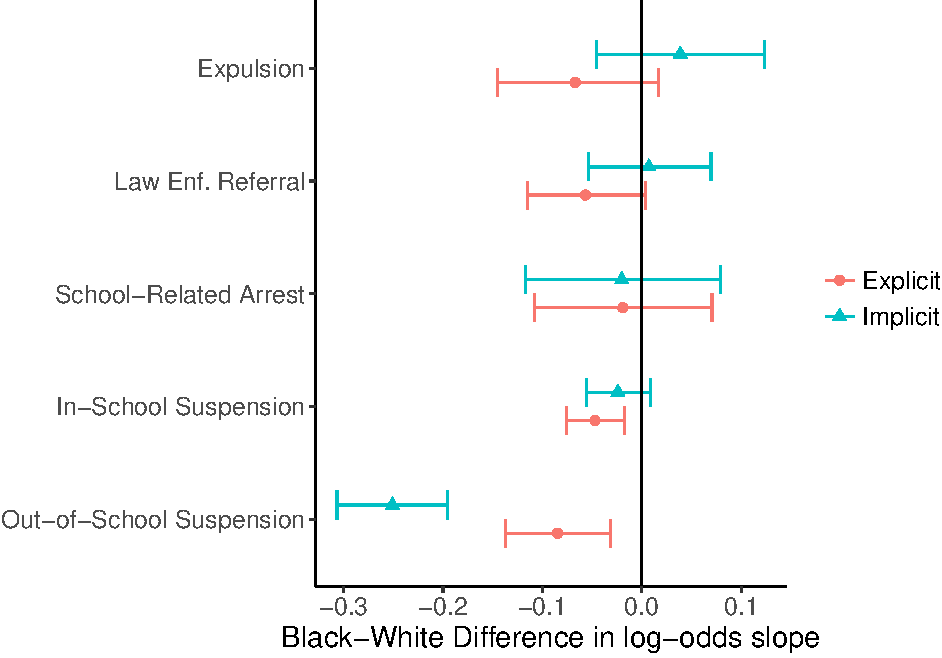
\includegraphics{draft_files/figure-latex/overall-associations-1.pdf}
\caption{\label{fig:overall-associations}Association between each metric and
county-level estimates of explicit and implicit bias. Negative values
indicate that the rate of increase (or decrease) for blacks is faster
(or slower) than for whites. Point is the mean of the posterior and
error bars represent 95\% bayesian uncertainty intervals.}
\end{figure}

Several patterns are apparent from this figure. First, in all cases but
school-related arrests, county-level explicit biases are reliably
associated with disciplinary disparities, such that counties with more
bias are expected to have a larger racial gap. The effect with the
largest magnitude of these is out-of-school suspensions (\(M_{slope}\) =
-0.12, {[}-0.18, -0.06{]}), followed by expulsions (\(M_{slope}\) =
-0.11, {[}-0.21, -0.01{]}), law enforcement referrals (\(M_{slope}\) =
-0.10, {[}-0.16, -0.03{]}), and in-school suspensions (\(M_{slope}\) =
-0.08, {[}-0.12, -0.05{]}). The model indicates that the evidence for
school-related arrests is inconclusive (\(M_{slope}\) = -0.03, {[}-0.13,
0.08{]}).

Second, the effect with the largest magnitude of all is that between
implicit biases and out-of-school suspension (\(M_{slope}\) = -0.22,
{[}-0.28, -0.16{]}). All other estimated parameters are inconclusive.

\begin{table}[tbp]
\begin{center}
\begin{threeparttable}
\caption{\label{tab:reg-coefs}Regression coefficient estimates for the population-level (i.e. fixed) effects, along with 95\% uncertainty intervals for each of the disciplinary metrics.}
\small{
\begin{tabular}{llllll}
\toprule
 & \multicolumn{1}{c}{Out-of-School Suspension} & \multicolumn{1}{c}{Law Enf. Referral} & \multicolumn{1}{c}{In-School Suspension} & \multicolumn{1}{c}{School-Related Arrest} & \multicolumn{1}{c}{Expulsion}\\
\midrule
Intercept & -2.02, [-2.07,-1.97] & -5.75, [-5.83,-5.67] & -2.3, [-2.33,-2.26] & -7.82, [-7.98,-7.66] & -6.5, [-6.6,-6.4]\\
total population & 0.01, [-0.02,0.03] & 0.03, [-0.03,0.09] & -0.04, [-0.07,-0.01] & 0.13, [0.04,0.22] & 0.03, [-0.04,0.11]\\
propotion black & 0.4, [0.31,0.49] & -0.25, [-0.46,-0.03] & 0.19, [0.09,0.3] & -0.14, [-0.5,0.24] & -0.13, [-0.38,0.12]\\
proportion white & 0.03, [-0.03,0.09] & -0.2, [-0.36,-0.04] & 0, [-0.08,0.08] & 0.02, [-0.26,0.3] & -0.2, [-0.39,-0.01]\\
black-white ratio & -0.26, [-0.32,-0.19] & 0.07, [-0.1,0.24] & -0.34, [-0.42,-0.27] & -0.09, [-0.38,0.18] & -0.18, [-0.39,0.01]\\
college grads & -0.03, [-0.06,0] & 0.03, [-0.05,0.11] & -0.09, [-0.13,-0.05] & 0.17, [0.04,0.31] & -0.12, [-0.22,-0.02]\\
income & -0.13, [-0.18,-0.08] & -0.08, [-0.2,0.03] & -0.13, [-0.18,-0.07] & 0.03, [-0.15,0.21] & -0.28, [-0.42,-0.14]\\
poverty & -0.06, [-0.13,0.01] & -0.63, [-0.81,-0.46] & 0.1, [0.01,0.18] & -0.29, [-0.59,0] & -0.4, [-0.61,-0.19]\\
unemployment & 0.23, [0.19,0.27] & 0.2, [0.1,0.29] & 0.03, [-0.01,0.07] & 0.3, [0.15,0.46] & 0.29, [0.19,0.39]\\
crime & 0.04, [0.01,0.07] & 0.07, [0,0.14] & 0.06, [0.03,0.09] & 0.11, [-0.01,0.22] & 0.09, [0.01,0.17]\\
housing density & -0.01, [-0.03,0.02] & -0.07, [-0.14,0.01] & 0, [-0.04,0.03] & -0.06, [-0.15,0.04] & 0, [-0.07,0.08]\\
mobility & 0.02, [-0.01,0.05] & 0.07, [0,0.14] & 0.01, [-0.02,0.04] & 0.05, [-0.07,0.17] & 0.01, [-0.07,0.1]\\
race: white & -0.65, [-0.69,-0.61] & -0.87, [-0.93,-0.81] & -0.85, [-0.87,-0.82] & -1.1, [-1.22,-0.99] & -0.93, [-1.01,-0.85]\\
implicit bias & 0.36, [0.29,0.43] & -0.1, [-0.23,0.02] & 0.21, [0.15,0.28] & -0.25, [-0.45,-0.05] & 0.03, [-0.12,0.18]\\
explicit bias & -0.05, [-0.11,0.02] & -0.01, [-0.13,0.1] & 0.1, [0.04,0.16] & 0.37, [0.19,0.55] & 0.04, [-0.09,0.18]\\
implicit bias*race: white & -0.22, [-0.28,-0.16] & 0.05, [-0.02,0.12] & 0.01, [-0.02,0.05] & -0.01, [-0.13,0.09] & 0.07, [-0.03,0.17]\\
explicit bias*race: white & -0.12, [-0.18,-0.06] & -0.1, [-0.16,-0.03] & -0.08, [-0.12,-0.05] & -0.03, [-0.13,0.08] & -0.11, [-0.2,-0.02]\\
\bottomrule
\end{tabular}
}
\end{threeparttable}
\end{center}
\end{table}

The findings for other disciplinary metrics suggest a differential
effect of explicit and implicit bias. For example, there is a reliable
association between in-school suspensions and explicit bias. The
difference in the slope of the association between explicit bias and the
log of the odds for in-school suspensions between white and black
students is estimated to be -0.12, with 95\% of the posterior
distribution between -0.18 and -0.06 and a proportion \textgreater{}.99
of the posterior distribution consistent with a negative effect. Similar
effects can be seen for explicit bias and law enforcement referrals
(-0.10, {[}-0.16, -0.03{]}, \(p_{neg}\) \textgreater{}.99), and explicit
bias and expulsions (-0.11, {[}-0.21, -0.01{]}, \(p_{neg}\) = .99). In
contrast, zero is included as a plausible value for the associations
between implicit bias and in-school suspensions (0.01, {[}-0.02,
0.05{]}, \(p_{neg}\) = .27), law enforcement referrals (0.05, {[}-0.02,
0.12{]}, \(p_{neg}\) = .08), and expulsions (0.07, {[}-0.03, 0.17{]},
\(p_{neg}\) = .07).

\begin{figure}
\centering
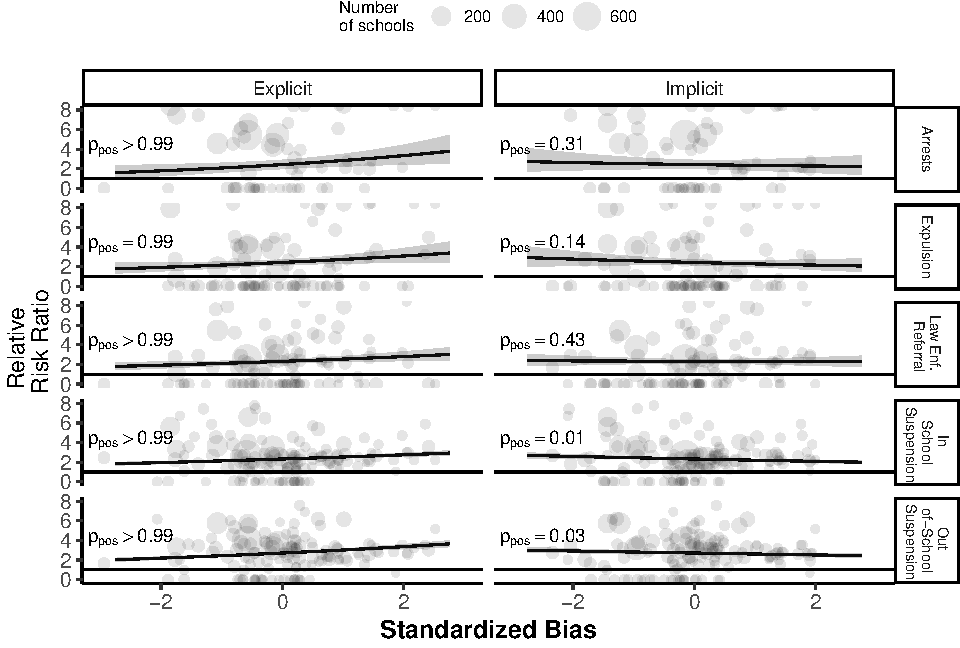
\includegraphics{draft_files/figure-latex/detail-risks-1.pdf}
\caption{\label{fig:detail-risks}Association between bias and relative risk
ratio for black students to white students. Line is the mean of the
posterior. Bands indicate 95\% uncertainty intervals. Points represent
counties, whose sizes are scaled to the number of schools in that
county. Note that the y axis is cut at 8 for legibility despite data
extending beyond.}
\end{figure}

To better illustrate the nature of these relationships, figure
\ref{fig:detail-risks} shows the estimated relative risk ratios for each
type of bias measurement and each disciplinary metric. Examining the
risk ratio for out-of-school suspensions, in a hypothetical county with
0 standardized bias on both implicit and explicit, the model predicts
that for every white student expelled, we should expect 1.81 {[}1.74,
1.88{]} black students to be expelled. If we move to a county one
standard deviation above the mean of explicit bias, the ratio of black
to white students expelled increases to 2.17 {[}2.05, 2.30{]}, while the
same movement for implicit bias increase the ratio to 2.03 {[}1.90,
2.17{]}.`

\begin{figure}
\centering
\includegraphics{draft_files/figure-latex/detail-rates-1.pdf}
\caption{\label{fig:detail-rates}Association between bias and probability of
receiving disciplinary action for black and white students. Lines are
the means of the posterior. Bands indicate 95\% uncertainty intervals.}
\end{figure}

Figure \ref{fig:detail-rates} unpacks these risk ratios by detailing the
probabilities of receiving disciplinary action as a function of race,
bias, and type of action. In a hypotheticl county with 0 standardized
bias on both implicit and explicit, the model predicts that 11.70\%
{[}11.20, 12.20{]} of black students will receive an out-of-school
suspension . The corresponding rate for white students is just over half
that for black students, with about 6.50\% {[}6.30, 6.60{]} expected to
be suspended. Holding all other variables constant, moving to a
hypothetical county one standard deviation above the mean of explicit
bias has the effect of slightly decreasing the estimated percentage of
black students expected to be suspended to 11.20\% {[}10.40, 12.10{]},
while the percentage of white students expected to be suspended would
decrease at a faster rate to 5.50\% {[}5.30, 5.80{]}. The same movement
for implicit bias would dramatically increase the expected suspensions
for black students (16\% {[}14.90, 17.10), and increase the expected
suspensions for white students a much smaller amount to (7.40\% {[}7,
7.70).

\section{Discussion}\label{discussion}

\newpage

\section{References}\label{references}

\newpage

\section{Appendix}\label{appendix}

\subsection{Session details}\label{session-details}

Data analysis was done in R (R Core Team, 2016) version 3.3.2 running
under OS X 10.11.6. Post-stratification was done with lme4, version
1.1.14 (Bates, Mächler, Bolker, \& Walker, 2015). Final model fitting
was done on the university cluster running Springdale Linux, release 6.9
using rstanarm, version 2.17.2 (Stan Development Team, 2016). We used
the implementation of the consensus monte carlo algorithm found in
parallelMCMCcombine, version 1.0 (Miroshnikov \& Conlon, 2014). Figures
were made with ggplot2, version 2.2.1 (Wickham, 2009), with data
manipulation done using dplyr version 0.7.2 (Wickham, Francois, Henry,
\& Müller, 2017) and tidyr, version 0.7.1 (Wickham \& Henry, 2017). A
full report of session information can be found on the OSF page
(\ldots{}.)

\subsection{Preregistered analysis}\label{preregistered-analysis}

Here, we describe, in detail, the differences between the registered
analysis plan and that presented in the main text, along with our
reasons for making the alterations.

\subsubsection{Data exclusions}\label{data-exclusions}

In our preanalysis plan, we specified our analyses to focus on 13
actions - corporal punishment, in-school suspension, out-of-school
suspension, expulsion with educational services, expulsion without
educational services, expulsion under zero-tolerance policies, referral
to law enforcement, school-related arrests, mechanical restraint,
physical restraint, seclusion, preschool suspension, and preschool
expulsion. However, upon further study, we discovered reasons we thought
justified excluding a number of these outcomes.

First, seclusion, physical restraint, and mechanical restraint are not
disciplinary actions, but are rather used as means to restrain students
who are at risk of harming themselves or others.

Next, we discovered that the administration of corporal punishment was
extremely irregular across counties, with almost all cases ocurring in
the South. Specifically, Alabama, Arkansas, Florida, Georgia, Louisiana,
Missouri, Mississippi, Oklahoma, Tennessee, and Texas accounted for 98\%
of all educational institutions that administered corporal punishment at
least once, despite containing only 26.90\% of the educational
institutions in the full dataset. It is not clear whether this uneven
distribution is due to legal prohibitions, cultural differences, or some
combination of the two. Because this makes interpretation of the
parameters uncertain, this analysis is also placed in the appendix.

We also found that the number of preschool students who are expelled or
suspended is vanishingly small (131 total expulsions and 6751 total
suspensions out of over 1.4 million enrolled preschool students), making
reliably estimating any association across counties exceedingly
unlikely. We additionally discovered that counts of one expulsion
category (expulsion under zero-tolerance policies) overlapped with
counts in other categories, and so excluded this category from the main
text. We also decided to combine the remaining two expulsion categories
to yield one overall count of the number of students expelled. We did
this to remain consistent with previous research, and to obtain
district-level rates of expulsion that were slightly higher, and
therefore more amenable to exploring variation across counties.

When preparing the preregistration, we also had not known about the
issues with juvenile justice facilities, or with the school districts
with reporting errors, and so excluded these schools from analyses in
the main text.

\subsubsection{Changes in measurement \& estimation of
bias}\label{changes-in-measurement-estimation-of-bias}

We preregistered our explicit bias as a simple feeling thermometer
towards balcks (i.e. \emph{how warm or cold do you feel towards Blacks?
0=very cold, 10=very warm}). However, the majority of past research (see
for example Leitner et al. (2016) and Hehman, Flake, and Calanchini
(2017)) has used the difference in reported warmth towards whites and
blacks, and so in the main text, we report models using this metric of
explicit bias.

Our main text presents analyses with poststratified estimates of bias.
Our registered analysis also described analyses with raw, county-based
means. Unlike previous papers that used poststratification, we see
substantial differences in results between the two estimation methods.
Because post-stratification is known to yield better estimates, we
suspect that the difference in results is largely driven by extreme
county-level observations with little data to support these extreme
estimates. Nevertheless, in the interest of completion, we present the
model using raw county-level means as well.

We also registered an exploratory analysis using the responses of people
who visited Project Implicit and identified themselves as teachers.
Unfortunately, without population-level data on the demographic
characteristics of teachers, we are not able to post-stratify these
estimates. Additionally, there were relatively few teachers in the
Project Implicit from which to derive estimates. Ultimately, we have
little confidence that this analysis tells us anything about whether the
biases of teachers specifically contribute to disparities in
disciplinary actions, and so this analysis is also limited to the
appendix.

\subsubsection{Additional covariates}\label{additional-covariates}

We included three covariates that were not specified in the registered
analysis. Specifically, the mobility, housing density, and crime rate
covariates. These covariates were included in order to cover more of the
covariates that were included in previous papers (Leitner et al., 2016).

\subsection{Registered analysis
results}\label{registered-analysis-results}

Here, we present the results of the preregistered analyses exactly.
Though we described a number of changes above, it is not practical to
run all possible combination of changes, as each set of models takes
four to five days to just to estimate, and there are at least several
dozen possible combinations of decisions to test, depending on how
fine-grained one wishes to be with the decisions. Accordingly, we limit
the presentation of results below to just the three models that we
registered.

\subsubsection{County-level estimates}\label{county-level-estimates}

\begin{figure}
\centering
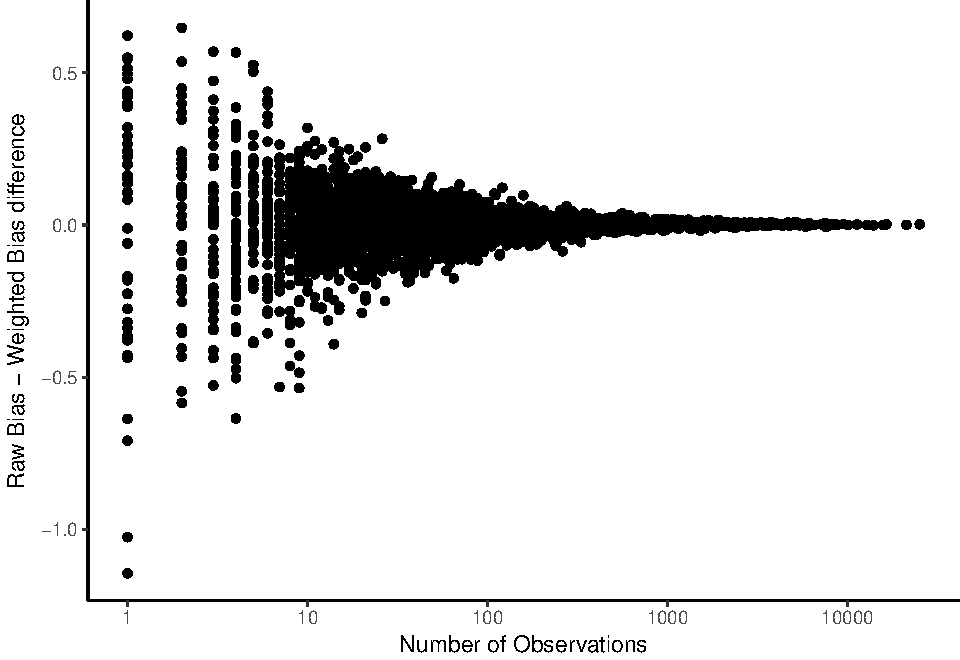
\includegraphics{draft_files/figure-latex/raw-county-estimates-1.pdf}
\caption{\label{fig:raw-county-estimates}Difference in raw county means and
post-stratifed estimates of implicit bias as a function of the number of
observations in each county. The X axis is on the log scale.}
\end{figure}

Examining the models fit with simple county means, we find that the
county-level estimates vary more than with the post-stratified
estimates. This pattern is expected, as one desireable feature of
post-stratification is that it regularizes extreme observations without
a large amount of data to support them. This phenomena is illustrated in
figure \ref{fig:raw-county-estimates}, which shows the distribution of
differences between the raw county means and the post-stratified
estimates of implicit bias as a function of the number of observations
in each county. More specifically, while the mean of the county-level
means does not meaningfully differ from the post-stratified estimates,
the standard deviation is much larger (\(M_{implicit}\) = 0.40,
\(SD_{implicit}\) = 0.11; \(M_{explicit}\) = 6.25, \(SD_{explicit}\) =
0.60)\footnote{This explicit estimate is based on the simple warmth
  towards blacks question, and not the difference between warmth towards
  whites and warmth twoards blacks.}

The county-level implicit bias estimates for the poststratified model
are as reported in the main text. The estimates for explicit bias are
slightly different, as they are not computed based on the difference in
reporting warmth toward whites and warmth toward blacks. Specifically,
the average amount of bias at the county-level is 6.26 (SD = 0.13).

A subset of years in the Project Implicit data also collected
occupational information from respondents. As identified in our
pre-analysis plan, we took advantage of the presence of primary and
secondary educators in these data to test whether any associations
between bias and race-based differences in the rates of disciplinary
action were stronger among these respondents. Filtering for only white
individuals who identified as primary, secondary, special education, and
other teachers and instructors (occupation codes 25-2000 and 25-3000)
reduced the dataset to 63552 respondents. In order to assure that our
estimates were reasonably stable, we limited analysis to only counties
that had at least 50 respondents. As such, our teacher analysis is
limited to just 287 counties. Additionally, because we do not know of
any state-level demographic estimates for teachers, we were unable to
perform post-stratification for these data. Nonetheless, across these
limited counties, the overall estimate of implicit and explicit bias are
similar to those for the whole dataset (\(M_{implicit}\) = 0.38,
\(SD_{implicit}\) = 0.06; \(M_{explicit}\) = -6.70, \(SD_{explicit}\) =
0.27)

\subsubsection{Model estimates}\label{model-estimates}

Table \ref{tab:mod-raw} presents results from the model fit to the raw,
county-level means. The table presents parameter estimates
(operationalized as the mean of the posterior) and 95\% uncertainty
intervals for each of the population-level effects for each of the
outcomes. Table \ref{tab:mod-post} and table \ref{tab:mod-teach} present
the corresponding results for the post-stratified and teacher models,
respectively.

\begin{lltable}
\small{
\begin{longtable}{llllllllllllll}\noalign{\getlongtablewidth\global\LTcapwidth=\longtablewidth}
\caption{\label{tab:mod-raw}Regression coefficient estimates for the population-level (i.e. fixed) effects, along with 95\% uncertainty intervals for each of the disciplinary metrics. Model uses raw, county-level means as estimates of implicit and explicit bias.}\\
\toprule
 & \multicolumn{1}{c}{Seclusion} & \multicolumn{1}{c}{Preschool Suspension} & \multicolumn{1}{c}{Preschool Expulsion} & \multicolumn{1}{c}{Physical Restraint} & \multicolumn{1}{c}{Out-of-School Suspension} & \multicolumn{1}{c}{Mechanical Restraint} & \multicolumn{1}{c}{Law Enf. Referral} & \multicolumn{1}{c}{In-School Suspension} & \multicolumn{1}{c}{School-Related Arrest} & \multicolumn{1}{c}{Expulsion without Educational Services} & \multicolumn{1}{c}{Expulsion with Educational Services} & \multicolumn{1}{c}{Expulsion Under Zero-Tolerance} & \multicolumn{1}{c}{Corporal Punishment}\\
\midrule
Intercept & -11.19, [-11.64,-10.77] & -8.84, [-9.15,-8.56] & -16.07, [-17.96,-14.35] & -8.78, [-8.99,-8.58] & -2.68, [-2.71,-2.65] & -14.1, [-14.96,-13.31] & -6.12, [-6.21,-6.03] & -2.63, [-2.67,-2.59] & -8.2, [-8.37,-8.04] & -8.22, [-8.39,-8.07] & -8.11, [-8.28,-7.94] & -9.74, [-10.01,-9.49] & -3.21, [-3.31,-3.13]\\
total population & 0.16, [0.01,0.31] & 0.05, [-0.07,0.17] & 0.49, [0.24,0.76] & 0.02, [-0.07,0.12] & 0.01, [-0.02,0.03] & 0.41, [0.2,0.65] & 0.01, [-0.06,0.07] & -0.03, [-0.07,0.01] & 0.09, [0,0.19] & 0.01, [-0.08,0.1] & 0.06, [-0.03,0.15] & 0.09, [-0.01,0.2] & -0.48, [-0.67,-0.3]\\
propotion black & -1.51, [-2.18,-0.85] & 1.02, [0.59,1.46] & 0.99, [-0.47,2.53] & -0.67, [-1.04,-0.3] & 0.34, [0.27,0.42] & 0.8, [-0.15,1.75] & -0.45, [-0.64,-0.25] & 0.61, [0.51,0.7] & -0.19, [-0.5,0.12] & 0.32, [0.04,0.61] & -0.29, [-0.62,0.02] & 0.02, [-0.36,0.42] & 0.11, [-0.14,0.37]\\
proportion white & 0.26, [-0.23,0.74] & -0.44, [-0.8,-0.07] & -0.34, [-1.53,0.91] & 0.19, [-0.08,0.45] & 0.02, [-0.03,0.08] & 0.26, [-0.48,1.06] & -0.34, [-0.48,-0.2] & 0.13, [0.05,0.2] & -0.06, [-0.31,0.19] & 0.23, [-0.03,0.49] & -0.25, [-0.47,-0.02] & 0.21, [-0.08,0.51] & -0.3, [-0.51,-0.08]\\
black-white ratio & 0.81, [0.17,1.45] & -0.78, [-1.14,-0.44] & -0.34, [-1.63,0.82] & 0.26, [-0.08,0.6] & -0.21, [-0.27,-0.15] & -0.59, [-1.5,0.27] & 0.06, [-0.1,0.22] & -0.53, [-0.62,-0.45] & 0.09, [-0.18,0.36] & -0.13, [-0.36,0.09] & -0.22, [-0.53,0.07] & -0.23, [-0.62,0.13] & -0.34, [-0.52,-0.15]\\
college grads & 0.25, [0.01,0.48] & -0.21, [-0.4,-0.01] & -0.24, [-0.98,0.45] & 0.3, [0.17,0.43] & -0.04, [-0.07,-0.01] & -0.04, [-0.46,0.37] & 0.03, [-0.06,0.11] & -0.12, [-0.16,-0.07] & 0.15, [0.02,0.29] & -0.2, [-0.34,-0.06] & -0.06, [-0.2,0.07] & -0.08, [-0.25,0.09] & -0.15, [-0.25,-0.05]\\
income & -0.32, [-0.64,-0.01] & -0.3, [-0.57,-0.03] & -0.35, [-1.27,0.55] & -0.18, [-0.36,0] & -0.09, [-0.13,-0.05] & 0, [-0.5,0.53] & -0.05, [-0.16,0.06] & -0.08, [-0.14,-0.02] & 0, [-0.18,0.18] & -0.31, [-0.49,-0.14] & -0.09, [-0.26,0.09] & -0.08, [-0.3,0.14] & -0.33, [-0.47,-0.18]\\
poverty & -0.64, [-1.05,-0.22] & -0.32, [-0.65,-0.01] & -1.21, [-2.46,0.02] & -0.14, [-0.38,0.09] & 0.02, [-0.03,0.08] & 0.3, [-0.32,0.95] & -0.4, [-0.54,-0.27] & 0.2, [0.13,0.27] & -0.22, [-0.44,0] & -0.35, [-0.56,-0.14] & -0.15, [-0.37,0.06] & 0.2, [-0.07,0.46] & 0.01, [-0.15,0.17]\\
unemployment & 0.4, [0.14,0.68] & -0.29, [-0.49,-0.1] & -0.3, [-1.08,0.48] & 0.23, [0.08,0.38] & 0.22, [0.18,0.25] & -0.21, [-0.64,0.24] & 0.19, [0.1,0.27] & 0.03, [-0.01,0.08] & 0.25, [0.1,0.39] & 0.45, [0.31,0.59] & 0.27, [0.13,0.41] & 0.31, [0.13,0.49] & -0.14, [-0.23,-0.04]\\
race: white & -1.04, [-1.39,-0.66] & -1.65, [-1.94,-1.36] & -1.91, [-3.47,-0.42] & -1.01, [-1.19,-0.82] & -1.06, [-1.09,-1.03] & -1.72, [-2.36,-1.09] & -0.83, [-0.9,-0.77] & -0.85, [-0.87,-0.82] & -1.07, [-1.19,-0.94] & -0.88, [-1.02,-0.74] & -0.85, [-0.99,-0.72] & -0.49, [-0.71,-0.26] & -0.68, [-0.73,-0.62]\\
implicit bias & -0.02, [-0.37,0.37] & -0.16, [-0.41,0.08] & 0.04, [-0.92,1.04] & 0, [-0.23,0.22] & 0.01, [-0.03,0.05] & -0.07, [-0.6,0.48] & -0.06, [-0.16,0.04] & 0.08, [0.03,0.12] & -0.09, [-0.27,0.1] & 0.04, [-0.12,0.21] & -0.1, [-0.29,0.08] & -0.03, [-0.26,0.2] & -0.01, [-0.11,0.08]\\
explicit bias & 0.33, [-0.04,0.69] & -0.17, [-0.41,0.06] & -0.05, [-1.12,0.94] & 0.07, [-0.13,0.28] & 0.03, [-0.01,0.07] & -0.14, [-0.65,0.36] & 0.09, [-0.01,0.2] & 0, [-0.05,0.04] & -0.02, [-0.18,0.15] & -0.01, [-0.17,0.15] & 0.02, [-0.15,0.2] & 0.3, [0.07,0.52] & -0.06, [-0.15,0.02]\\
implicit bias*race: white & 0.12, [-0.24,0.46] & 0.2, [-0.06,0.47] & -0.03, [-1.25,1.16] & 0.08, [-0.15,0.3] & -0.01, [-0.04,0.03] & 0.06, [-0.43,0.57] & -0.03, [-0.12,0.06] & -0.04, [-0.07,-0.01] & 0.01, [-0.16,0.17] & -0.09, [-0.24,0.05] & 0.11, [-0.04,0.25] & -0.19, [-0.42,0.04] & -0.04, [-0.1,0.04]\\
explicit bias*race: white & -0.22, [-0.57,0.14] & 0.08, [-0.18,0.34] & -0.4, [-1.66,0.91] & -0.01, [-0.21,0.2] & 0, [-0.03,0.03] & -0.09, [-0.59,0.43] & -0.1, [-0.19,-0.01] & -0.02, [-0.05,0.01] & -0.02, [-0.17,0.12] & 0, [-0.14,0.14] & -0.02, [-0.17,0.12] & -0.14, [-0.35,0.07] & 0, [-0.06,0.06]\\
\bottomrule
\end{longtable}
}
\end{lltable}

\begin{lltable}
\small{
\begin{longtable}{llllllllllllll}\noalign{\getlongtablewidth\global\LTcapwidth=\longtablewidth}
\caption{\label{tab:mod-post}Regression coefficient estimates for the population-level (i.e. fixed) effects, along with 95\% uncertainty intervals for each of the disciplinary metrics. Model uses poststratified estimates of implicit and explicit bias.}\\
\toprule
 & \multicolumn{1}{c}{Seclusion} & \multicolumn{1}{c}{Preschool Suspension} & \multicolumn{1}{c}{Preschool Expulsion} & \multicolumn{1}{c}{Physical Restraint} & \multicolumn{1}{c}{Out-of-School Suspension} & \multicolumn{1}{c}{Mechanical Restraint} & \multicolumn{1}{c}{Law Enf. Referral} & \multicolumn{1}{c}{In-School Suspension} & \multicolumn{1}{c}{School-Related Arrest} & \multicolumn{1}{c}{Expulsion without Educational Services} & \multicolumn{1}{c}{Expulsion with Educational Services} & \multicolumn{1}{c}{Expulsion Under Zero-Tolerance} & \multicolumn{1}{c}{Corporal Punishment}\\
\midrule
Intercept & -11.11, [-11.56,-10.7] & -9, [-9.34,-8.7] & -14.17, [-15.91,-12.61] & -8.73, [-8.94,-8.52] & -2.69, [-2.72,-2.66] & -13.96, [-14.8,-13.19] & -6.12, [-6.21,-6.04] & -2.63, [-2.67,-2.59] & -8.19, [-8.36,-8.03] & -8.2, [-8.36,-8.03] & -8.09, [-8.26,-7.92] & -9.66, [-9.92,-9.41] & -3.24, [-3.34,-3.15]\\
unemployment & 0.44, [0.18,0.71] & -0.21, [-0.4,-0.01] & -0.21, [-0.98,0.57] & 0.26, [0.11,0.41] & 0.21, [0.18,0.25] & -0.17, [-0.62,0.29] & 0.18, [0.09,0.26] & 0.06, [0.01,0.1] & 0.26, [0.11,0.41] & 0.41, [0.27,0.55] & 0.27, [0.13,0.41] & 0.26, [0.09,0.44] & -0.12, [-0.21,-0.02]\\
college grads & 0.2, [-0.04,0.45] & -0.12, [-0.32,0.08] & -0.2, [-0.92,0.49] & 0.27, [0.14,0.41] & -0.04, [-0.07,-0.01] & -0.02, [-0.44,0.4] & -0.01, [-0.1,0.07] & -0.08, [-0.12,-0.03] & 0.17, [0.04,0.31] & -0.23, [-0.37,-0.09] & -0.05, [-0.19,0.08] & -0.14, [-0.31,0.03] & -0.12, [-0.22,-0.02]\\
proportion white & 0.49, [0.02,0.98] & -0.56, [-0.92,-0.18] & -0.7, [-1.84,0.51] & 0.28, [0.01,0.56] & 0, [-0.06,0.06] & 0.18, [-0.58,1.02] & -0.29, [-0.44,-0.14] & 0.07, [-0.01,0.15] & -0.1, [-0.35,0.16] & 0.28, [0.01,0.54] & -0.26, [-0.5,-0.03] & 0.27, [-0.03,0.57] & -0.25, [-0.48,-0.02]\\
black-white ratio & 0.52, [-0.08,1.05] & -0.76, [-1.14,-0.41] & -0.37, [-1.86,0.9] & 0.15, [-0.25,0.54] & -0.19, [-0.24,-0.13] & -0.84, [-1.92,0.18] & -0.01, [-0.18,0.15] & -0.36, [-0.44,-0.28] & 0.08, [-0.17,0.33] & -0.19, [-0.42,0.04] & -0.17, [-0.47,0.11] & -0.24, [-0.62,0.11] & -0.33, [-0.52,-0.14]\\
race: white & -1.06, [-1.41,-0.67] & -1.6, [-1.92,-1.27] & -2.09, [-3.64,-0.56] & -1.02, [-1.2,-0.83] & -1.05, [-1.08,-1.02] & -1.77, [-2.43,-1.13] & -0.83, [-0.89,-0.76] & -0.84, [-0.86,-0.81] & -1.05, [-1.18,-0.92] & -0.9, [-1.04,-0.76] & -0.87, [-1,-0.73] & -0.53, [-0.75,-0.29] & -0.64, [-0.7,-0.58]\\
poverty & -0.55, [-0.97,-0.14] & -0.44, [-0.76,-0.11] & -1.02, [-2.23,0.14] & -0.14, [-0.37,0.1] & 0.02, [-0.03,0.07] & 0.3, [-0.36,0.93] & -0.38, [-0.52,-0.24] & 0.16, [0.1,0.23] & -0.2, [-0.43,0.02] & -0.3, [-0.52,-0.09] & -0.17, [-0.39,0.05] & 0.23, [-0.04,0.49] & 0, [-0.16,0.16]\\
total population & 0.14, [0,0.28] & 0.03, [-0.06,0.13] & 0.22, [0.01,0.45] & 0.03, [-0.05,0.11] & 0, [-0.03,0.02] & 0.32, [0.14,0.52] & 0.02, [-0.04,0.08] & -0.04, [-0.07,0] & 0.09, [0,0.18] & 0, [-0.08,0.09] & 0.06, [-0.03,0.16] & 0.09, [-0.02,0.2] & -0.44, [-0.62,-0.25]\\
implicit bias & -0.42, [-0.7,-0.14] & 0.14, [-0.09,0.39] & 0.01, [-0.97,1.07] & -0.33, [-0.5,-0.16] & 0.08, [0.04,0.13] & -0.07, [-0.53,0.43] & -0.08, [-0.18,0.02] & 0.13, [0.08,0.19] & 0, [-0.16,0.16] & -0.03, [-0.19,0.12] & -0.03, [-0.2,0.13] & -0.15, [-0.35,0.06] & 0.01, [-0.11,0.14]\\
implicit bias*race: white & -0.1, [-0.33,0.11] & -0.06, [-0.28,0.15] & -0.72, [-1.97,0.5] & 0.18, [0.05,0.31] & -0.04, [-0.06,-0.01] & -0.02, [-0.39,0.35] & -0.04, [-0.1,0.02] & -0.04, [-0.07,-0.01] & 0, [-0.1,0.09] & -0.02, [-0.12,0.09] & 0.09, [-0.01,0.18] & 0.07, [-0.08,0.22] & -0.11, [-0.18,-0.05]\\
propotion black & -0.79, [-1.46,-0.11] & 0.78, [0.33,1.25] & 0.58, [-0.87,2.16] & -0.4, [-0.81,0.02] & 0.28, [0.21,0.36] & 0.86, [-0.2,1.92] & -0.28, [-0.48,-0.07] & 0.31, [0.2,0.41] & -0.26, [-0.58,0.07] & 0.47, [0.15,0.8] & -0.37, [-0.69,-0.03] & 0.17, [-0.24,0.59] & 0.13, [-0.17,0.42]\\
explicit bias & 0.11, [-0.15,0.37] & -0.21, [-0.41,-0.02] & -0.51, [-1.39,0.42] & -0.04, [-0.2,0.13] & 0.06, [0.02,0.09] & -0.06, [-0.48,0.36] & 0.12, [0.03,0.21] & -0.16, [-0.2,-0.11] & -0.08, [-0.23,0.06] & 0.14, [0,0.28] & -0.06, [-0.2,0.08] & 0.25, [0.07,0.43] & -0.14, [-0.25,-0.04]\\
explicit bias*race: white & -0.15, [-0.36,0.07] & -0.13, [-0.32,0.06] & -0.48, [-1.66,0.62] & 0.03, [-0.11,0.17] & 0, [-0.02,0.03] & -0.32, [-0.66,0.03] & -0.04, [-0.1,0.01] & 0, [-0.03,0.02] & -0.02, [-0.11,0.07] & 0.02, [-0.08,0.11] & 0.04, [-0.05,0.12] & 0.02, [-0.12,0.16] & -0.02, [-0.08,0.04]\\
income & -0.27, [-0.58,0.03] & -0.38, [-0.65,-0.11] & -0.15, [-1.06,0.75] & -0.17, [-0.35,0.01] & -0.09, [-0.14,-0.05] & 0.03, [-0.49,0.54] & -0.03, [-0.14,0.08] & -0.11, [-0.16,-0.05] & -0.01, [-0.18,0.17] & -0.29, [-0.47,-0.11] & -0.11, [-0.28,0.07] & -0.06, [-0.28,0.16] & -0.38, [-0.53,-0.22]\\
\bottomrule
\end{longtable}
}
\end{lltable}

\begin{lltable}
\small{
\begin{longtable}{llllllllllllll}\noalign{\getlongtablewidth\global\LTcapwidth=\longtablewidth}
\caption{\label{tab:mod-teach}Regression coefficient estimates for the population-level (i.e. fixed) effects, along with 95\% uncertainty intervals for each of the disciplinary metrics. Model uses only data from Project Implicit respondents who identified as teachers.}\\
\toprule
 & \multicolumn{1}{c}{Seclusion} & \multicolumn{1}{c}{Preschool Suspension} & \multicolumn{1}{c}{Preschool Expulsion} & \multicolumn{1}{c}{Physical Restraint} & \multicolumn{1}{c}{Out-of-School Suspension} & \multicolumn{1}{c}{Mechanical Restraint} & \multicolumn{1}{c}{Law Enf. Referral} & \multicolumn{1}{c}{In-School Suspension} & \multicolumn{1}{c}{School-Related Arrest} & \multicolumn{1}{c}{Expulsion without Educational Services} & \multicolumn{1}{c}{Expulsion with Educational Services} & \multicolumn{1}{c}{Expulsion Under Zero-Tolerance} & \multicolumn{1}{c}{Corporal Punishment}\\
\midrule
Intercept & -10.12, [-10.63,-9.66] & -8.6, [-9.04,-8.21] & -13.68, [-15.54,-12.13] & -8.22, [-8.46,-8] & -2.34, [-2.4,-2.29] & -12.87, [-13.88,-11.99] & -5.57, [-5.7,-5.44] & -2.7, [-2.77,-2.62] & -7.31, [-7.55,-7.07] & -8.41, [-8.72,-8.09] & -7.61, [-7.86,-7.36] & -9.38, [-9.72,-9.06] & -6.25, [-7.29,-5.37]\\
poverty & -0.33, [-1.31,0.63] & 0.31, [-0.45,1.04] & 0.39, [-1.6,2.26] & -0.01, [-0.51,0.47] & -0.06, [-0.17,0.04] & 0.41, [-0.99,1.8] & -0.26, [-0.53,0] & 0.05, [-0.1,0.21] & 0.08, [-0.43,0.57] & -0.12, [-0.82,0.56] & 0.28, [-0.19,0.73] & 0.4, [-0.17,0.95] & -0.16, [-2.01,1.48]\\
college grads & 0.14, [-0.36,0.66] & -0.1, [-0.5,0.31] & -0.3, [-1.69,0.99] & 0.33, [0.08,0.58] & -0.15, [-0.22,-0.08] & -0.5, [-1.27,0.27] & -0.03, [-0.2,0.13] & -0.26, [-0.36,-0.15] & 0, [-0.29,0.27] & -0.16, [-0.52,0.2] & -0.22, [-0.52,0.07] & -0.25, [-0.63,0.11] & -0.11, [-1.01,0.78]\\
proportion white & 1.5, [0.46,2.52] & 0.25, [-0.66,1.16] & 1.39, [-0.37,3.33] & 0.74, [0.24,1.25] & 0.07, [-0.04,0.19] & 0.79, [-0.7,2.31] & -0.29, [-0.56,-0.01] & 0.23, [0.06,0.4] & 0.31, [-0.21,0.85] & 0.81, [0.14,1.5] & 0.2, [-0.29,0.7] & 0.17, [-0.48,0.83] & -1.73, [-4.31,0.84]\\
black-white ratio & 0.18, [-1.4,1.69] & -0.51, [-1.2,0.16] & -1.76, [-3.74,0.07] & -0.01, [-0.65,0.63] & -0.08, [-0.18,0.03] & -1.82, [-3.66,-0.06] & 0.07, [-0.3,0.44] & -0.32, [-0.49,-0.16] & 0.27, [-0.5,0.99] & 0.04, [-0.62,0.73] & -0.09, [-0.74,0.54] & -0.01, [-1.09,1.04] & -0.85, [-2.88,0.99]\\
implicit bias & -0.38, [-0.97,0.21] & 0.15, [-0.32,0.63] & -1.04, [-2.7,0.62] & -0.4, [-0.72,-0.07] & -0.02, [-0.11,0.06] & -0.65, [-1.64,0.3] & 0.08, [-0.12,0.27] & -0.02, [-0.13,0.09] & -0.07, [-0.43,0.29] & -0.2, [-0.62,0.23] & -0.56, [-0.94,-0.18] & -0.15, [-0.59,0.28] & 0.09, [-1.2,1.47]\\
explicit bias*race: white & 0.11, [-0.27,0.48] & -0.12, [-0.57,0.31] & -2.05, [-4.45,0.26] & 0.11, [-0.12,0.34] & -0.01, [-0.06,0.05] & -0.68, [-1.51,0.1] & 0.03, [-0.07,0.14] & -0.01, [-0.06,0.05] & 0, [-0.18,0.16] & -0.25, [-0.46,-0.04] & -0.04, [-0.22,0.13] & -0.07, [-0.34,0.21] & -0.21, [-0.98,0.51]\\
income & -0.4, [-1.23,0.39] & -0.21, [-0.91,0.49] & 1.4, [-0.21,3] & -0.42, [-0.84,-0.01] & -0.23, [-0.33,-0.13] & -0.13, [-1.45,1.13] & -0.37, [-0.6,-0.13] & -0.2, [-0.36,-0.05] & -0.05, [-0.49,0.4] & -0.53, [-1.15,0.05] & 0.11, [-0.34,0.57] & -0.11, [-0.69,0.41] & -0.38, [-1.72,0.95]\\
total population & 0.35, [0.01,0.72] & 0.16, [-0.16,0.47] & 0.43, [-0.06,0.94] & 0.02, [-0.19,0.23] & -0.05, [-0.12,0.01] & 0.66, [0.11,1.25] & -0.02, [-0.16,0.12] & 0, [-0.1,0.09] & 0.09, [-0.14,0.33] & 0.12, [-0.16,0.4] & 0.06, [-0.22,0.33] & 0.07, [-0.19,0.34] & -0.97, [-2.25,0.07]\\
explicit bias & 0.12, [-0.43,0.66] & 0.05, [-0.45,0.56] & -0.07, [-1.32,1.22] & -0.2, [-0.51,0.13] & 0.04, [-0.03,0.12] & 0.81, [-0.11,1.8] & 0.09, [-0.1,0.28] & 0, [-0.11,0.11] & -0.05, [-0.4,0.31] & 0.08, [-0.34,0.5] & -0.05, [-0.43,0.32] & 0.07, [-0.37,0.52] & 0.51, [-0.71,1.75]\\
propotion black & 0.51, [-0.79,1.84] & 1.2, [0.27,2.13] & 2.88, [0.86,4.95] & 0.06, [-0.55,0.68] & 0.12, [-0.01,0.26] & 1.98, [0.19,3.79] & -0.58, [-0.97,-0.21] & 0.49, [0.29,0.69] & -0.25, [-1,0.51] & 0.22, [-0.55,0.99] & -0.4, [-1.04,0.26] & -0.6, [-1.54,0.31] & 0.02, [-2.7,3.11]\\
unemployment & -0.17, [-0.69,0.37] & -0.55, [-0.98,-0.15] & -0.04, [-1.06,1.05] & -0.07, [-0.33,0.2] & 0.11, [0.04,0.18] & -0.8, [-1.65,0.06] & 0.04, [-0.12,0.21] & -0.09, [-0.19,0.02] & 0.12, [-0.17,0.41] & 0.36, [-0.02,0.73] & 0.11, [-0.21,0.43] & 0.02, [-0.36,0.39] & -0.77, [-1.76,0.11]\\
race: white & -1.34, [-1.71,-0.97] & -1.63, [-2.07,-1.24] & -3.01, [-5.02,-1.01] & -1.13, [-1.31,-0.93] & -1.46, [-1.5,-1.42] & -1.38, [-2.13,-0.55] & -1.01, [-1.09,-0.93] & -1.14, [-1.18,-1.1] & -1.1, [-1.24,-0.95] & -1.07, [-1.25,-0.87] & -1.06, [-1.21,-0.92] & -0.72, [-0.96,-0.46] & -0.53, [-1.16,0.12]\\
implicit bias*race: white & 0.01, [-0.4,0.41] & -0.27, [-0.69,0.14] & 0.43, [-2.21,2.98] & 0.21, [-0.03,0.45] & 0, [-0.06,0.05] & 0.18, [-0.67,1.05] & -0.07, [-0.18,0.03] & 0, [-0.06,0.05] & 0.04, [-0.13,0.2] & -0.16, [-0.36,0.04] & -0.02, [-0.2,0.17] & -0.1, [-0.38,0.18] & -0.01, [-0.69,0.72]\\
\bottomrule
\end{longtable}
}
\end{lltable}

\setlength{\parindent}{-0.5in} \setlength{\leftskip}{0.5in}

\hypertarget{refs}{}
\hypertarget{ref-anyon2014persistent}{}
Anyon, Y., Jenson, J. M., Altschul, I., Farrar, J., McQueen, J., Greer,
E., \ldots{} Simmons, J. (2014). The persistent effect of race and the
promise of alternatives to suspension in school discipline outcomes.
\emph{Children and Youth Services Review}, \emph{44}, 379--386.

\hypertarget{ref-aud2011america}{}
Aud, S., KewalRamani, A., \& Frohlich, L. (2011). America's youth:
Transitions to adulthood. nces 2012-026. \emph{National Center for
Education Statistics}.

\hypertarget{ref-bates2015fitting}{}
Bates, D., Mächler, M., Bolker, B., \& Walker, S. (2015). Fitting linear
mixed-effects models using lme4. \emph{Journal of Statistical Software},
\emph{67}(1), 1--48.
doi:\href{https://doi.org/10.18637/jss.v067.i01}{10.18637/jss.v067.i01}

\hypertarget{ref-cuellar2015school}{}
Cuellar, A. E., \& Markowitz, S. (2015). School suspension and the
school-to-prison pipeline. \emph{International Review of Law and
Economics}, \emph{43}, 98--106.

\hypertarget{ref-friese2009and}{}
Friese, M., Hofmann, W., \& Schmitt, M. (2009). When and why do implicit
measures predict behaviour? Empirical evidence for the moderating role
of opportunity, motivation, and process reliance. \emph{European Review
of Social Psychology}, \emph{19}(1), 285--338.

\hypertarget{ref-galdi2008automatic}{}
Galdi, S., Arcuri, L., \& Gawronski, B. (2008). Automatic mental
associations predict future choices of undecided decision-makers.
\emph{Science}, \emph{321}(5892), 1100--1102.

\hypertarget{ref-gawronski2003implicit}{}
Gawronski, B., Geschke, D., \& Banse, R. (2003). Implicit bias in
impression formation: Associations influence the construal of
individuating information. \emph{European Journal of Social Psychology},
\emph{33}(5), 573--589.

\hypertarget{ref-gelman1997poststratification}{}
Gelman, A., \& Little, T. C. (1997). Poststratification into many
categories using hierarchical logistic regression. \emph{Survey
Methodology}, \emph{23}(2), 127--35.

\hypertarget{ref-gonsalkorale2009aging}{}
Gonsalkorale, K., Sherman, J. W., \& Klauer, K. C. (2009). Aging and
prejudice: Diminished regulation of automatic race bias among older
adults. \emph{Journal of Experimental Social Psychology}, \emph{45}(2),
410--414.

\hypertarget{ref-gregory2008discipline}{}
Gregory, A., \& Weinstein, R. S. (2008). The discipline gap and african
americans: Defiance or cooperation in the high school classroom.
\emph{Journal of School Psychology}, \emph{46}(4), 455--475.

\hypertarget{ref-gregory1995crime}{}
Gregory, J. F. (1995). The crime of punishment: Racial and gender
disparities in the use of corporal punishment in us public schools.
\emph{Journal of Negro Education}, 454--462.

\hypertarget{ref-haight2014ecological}{}
Haight, W., Gibson, P. A., Kayama, M., Marshall, J. M., \& Wilson, R.
(2014). An ecological-systems inquiry into racial disproportionalities
in out-of-school suspensions from youth, caregiver and educator
perspectives. \emph{Children and Youth Services Review}, \emph{46},
128--138.

\hypertarget{ref-hehman2017disproportionate}{}
Hehman, E., Flake, J. K., \& Calanchini, J. (2017). Disproportionate use
of lethal force in policing is associated with regional racial biases of
residents. \emph{Social Psychological and Personality Science},
1948550617711229.

\hypertarget{ref-hirschfield2009another}{}
Hirschfield, P. (2009). Another way out: The impact of juvenile arrests
on high school dropout. \emph{Sociology of Education}, \emph{82}(4),
368--393.

\hypertarget{ref-hofmann2005meta}{}
Hofmann, W., Gawronski, B., Gschwendner, T., Le, H., \& Schmitt, M.
(2005). A meta-analysis on the correlation between the implicit
association test and explicit self-report measures. \emph{Personality
and Social Psychology Bulletin}, \emph{31}(10), 1369--1385.

\hypertarget{ref-kinsler2011understanding}{}
Kinsler, J. (2011). Understanding the black--white school discipline
gap. \emph{Economics of Education Review}, \emph{30}(6), 1370--1383.

\hypertarget{ref-leitner2016blacks}{}
Leitner, J. B., Hehman, E., Ayduk, O., \& Mendoza-Denton, R. (2016).
Blacks' death rate due to circulatory diseases is positively related to
whites' explicit racial bias: A nationwide investigation using project
implicit. \emph{Psychological Science}, \emph{27}(10), 1299--1311.

\hypertarget{ref-losen2015we}{}
Losen, D. J., Hodson, C. L., Keith, I., Michael, A., Morrison, K., \&
Belway, S. (2015). Are we closing the school discipline gap?

\hypertarget{ref-matjasko2011effective}{}
Matjasko, J. L. (2011). How effective are severe disciplinary policies?
School policies and offending from adolescence into young adulthood.
\emph{Journal of School Psychology}, \emph{49}(5), 555--572.

\hypertarget{ref-mcconnell2001relations}{}
McConnell, A. R., \& Leibold, J. M. (2001). Relations among the implicit
association test, discriminatory behavior, and explicit measures of
racial attitudes. \emph{Journal of Experimental Social Psychology},
\emph{37}(5), 435--442.

\hypertarget{ref-miroshnikov2014parallel}{}
Miroshnikov, A., \& Conlon, E. (2014). \emph{ParallelMCMCcombine:
Methods for combining independent subset markov chain monte carlo (mcmc)
posterior samples to estimate a posterior density given the full data
set}. Retrieved from
\url{https://CRAN.R-project.org/package=parallelMCMCcombine}

\hypertarget{ref-nosek2011implicit}{}
Nosek, B. A., Hawkins, C. B., \& Frazier, R. S. (2011). Implicit social
cognition: From measures to mechanisms. \emph{Trends in Cognitive
Sciences}, \emph{15}(4), 152--159.

\hypertarget{ref-okonofua2016vicious}{}
Okonofua, J. A., Walton, G. M., \& Eberhardt, J. L. (2016). A vicious
cycle: A social--psychological account of extreme racial disparities in
school discipline. \emph{Perspectives on Psychological Science},
\emph{11}(3), 381--398.

\hypertarget{ref-pager2009sequencing}{}
Pager, D., Western, B., \& Sugie, N. (2009). Sequencing disadvantage:
Barriers to employment facing young black and white men with criminal
records. \emph{The ANNALS of the American Academy of Political and
Social Science}, \emph{623}(1), 195--213.

\hypertarget{ref-park2004bayesian}{}
Park, D. K., Gelman, A., \& Bafumi, J. (2004). Bayesian multilevel
estimation with poststratification: State-level estimates from national
polls. \emph{Political Analysis}, \emph{12}(4), 375--385.

\hypertarget{ref-pascoe2009perceived}{}
Pascoe, E. A., \& Smart Richman, L. (2009). Perceived discrimination and
health: A meta-analytic review. \emph{Psychological Bulletin},
\emph{135}(4), 531.

\hypertarget{ref-rcitation}{}
R Core Team. (2016). \emph{R: A language and environment for statistical
computing}. Vienna, Austria: R Foundation for Statistical Computing.
Retrieved from \url{https://www.R-project.org/}

\hypertarget{ref-scott2016bayes}{}
Scott, S. L., Blocker, A. W., Bonassi, F. V., Chipman, H. A., George, E.
I., \& McCulloch, R. E. (2016). Bayes and big data: The consensus monte
carlo algorithm. \emph{International Journal of Management Science and
Engineering Management}, \emph{11}(2), 78--88.

\hypertarget{ref-rstanarm2016}{}
Stan Development Team. (2016). Rstanarm: Bayesian applied regression
modeling via Stan. Retrieved from \url{http://mc-stan.org/}

\hypertarget{ref-wickham2009ggplot2}{}
Wickham, H. (2009). \emph{Ggplot2: Elegant graphics for data analysis}.
Springer-Verlag New York. Retrieved from \url{http://ggplot2.org}

\hypertarget{ref-wickham2017tidyr}{}
Wickham, H., \& Henry, L. (2017). \emph{Tidyr: Easily tidy data with
'spread()' and 'gather()' functions}. Retrieved from
\url{https://CRAN.R-project.org/package=tidyr}

\hypertarget{ref-wickham2017dplyr}{}
Wickham, H., Francois, R., Henry, L., \& Müller, K. (2017). \emph{Dplyr:
A grammar of data manipulation}. Retrieved from
\url{https://CRAN.R-project.org/package=dplyr}

\hypertarget{ref-xu2014psychology}{}
Xu, K., Nosek, B., \& Greenwald, A. (2014). Psychology data from the
race implicit association test on the project implicit demo website.
\emph{Journal of Open Psychology Data}, \emph{2}(1).

\hypertarget{ref-yeager2017loss}{}
Yeager, D. S., Purdie-Vaughns, V., Hooper, S. Y., \& Cohen, G. L.
(2017). Loss of institutional trust among racial and ethnic minority
adolescents: A consequence of procedural injustice and a cause of
life-span outcomes. \emph{Child Development}, \emph{88}(2), 658--676.






\end{document}
